\section{Véc-tơ trong mặt phẳng tọa độ}

\subsection{Đề 1}
\Opensolutionfile{ans}[ans/ans-0-B1]
\caulc
\begin{ex}%[0H9N1-2]
	Cho hai véc-tơ $\overrightarrow{a}=(1;2)$; $\overrightarrow{b}=(3;4)$. Tọa độ $\overrightarrow{c}=4\overrightarrow{a}-\overrightarrow{b}$
	\choice
	{\True $(1;4)$}
	{$(-1;4)$}
	{$(4;1)$}
	{$(-1;-4)$}
	\loigiai{
		Ta có $4\overrightarrow{a}=(4;8)$ nên $\vec{c}=4\vec{a}-\overrightarrow{b}=(4-3;8-4)=(1;4)$.}
\end{ex}

\begin{ex}%[0H9H1-3] 
	Cho tam giác $ABC$ với $A(1;4)$, $B(-2;2)$, $C(4;0)$. Tìm tọa độ véc-tơ $\overrightarrow{AM}$ với $M$ là trung điểm $BC$.
	\choice
	{$\overrightarrow{AM}=(-3;0)$}
	{$\overrightarrow{AM}=(0;3)$}
	{\True $\overrightarrow{AM}=(0;-3)$}
	{$\overrightarrow{AM}=(3;0)$}
	\loigiai{
		Vì $M$ là trung điểm $BC$ nên $\heva{&x_M=\dfrac{x_C+x_B}{2} \\&y_M=\dfrac{y_C+y_B}{2}}\Leftrightarrow \heva{&x_M=1 \\&y_M=1}$. Suy ra $\overrightarrow{AM}=(0;-3)$.}
\end{ex}

\begin{ex}%[0H9H1-4]
	Giá trị của $m$ sao cho $\overrightarrow{a}=(2m-1;3m)$ cùng phương $\overrightarrow{b}=(1;1)$ là
	\choice
	{$-2$}
	{$1$}
	{$-3$}
	{\True $-1$}
	\loigiai{
		$\overrightarrow{a}=(2m-1;3m)$ cùng phương $\overrightarrow{b}=(1;1)$ khi và chỉ khi $$\dfrac{2m-1}{1}=\dfrac{3m}{1}\Leftrightarrow 2m-1=3m\Leftrightarrow m=-1.$$}
\end{ex}

\begin{ex}%[0H9N1-1]
	Trong mặt phẳng với hệ tọa độ $Oxy$, cho hai điểm $A(2;-5)$ và $B(4;1)$. Tọa độ trung điểm $I$ của đoạn thẳng $AB$ là
	\choice
	{\True $I(3;-2)$}
	{$I(3;2)$}
	{$I(1;3)$}
	{$I(-1;-3)$}
	\loigiai{
		Tọa độ trung điểm $I$ của đoạn thẳng $AB$ là $\heva{&x_I=\dfrac{x_A+x_B}{2} \\&y_I=\dfrac{y_A+y_B}{2}}\Leftrightarrow \heva{&x_I=3 \\&y_I=-2}\Rightarrow I(3;-2)$.}
\end{ex}

\begin{ex}%[0H9N1-1]
	Trong mặt phẳng $Oxy$, cho ba điểm $A(2;0)$, $B(-1;-2)$, $C(5;-7)$. Tọa độ trọng tâm của $\Delta ABC$ là
	\choice
	{$(2;3)$}
	{\True $(2;-3)$}
	{$(3;2)$}
	{$(-3;2)$}
	\loigiai{
		Gọi $G$ là trọng tâm của $\Delta ABC$, ta có $\heva{&x_G=\dfrac{x_A+x_B+x_C}{3}=2 \\&y_G=\dfrac{y_A+y_B+y_C}{3}=-3}\Rightarrow G(2;-3)$.}
\end{ex}

\begin{ex}%[0H9H1-1]
	Trong hệ trục $\left(O;\overrightarrow{i};\overrightarrow{j}\right)$, cho véc-tơ $\overrightarrow{OM}=3\left(\overrightarrow{i}+4\overrightarrow{j}\right)+5\overrightarrow{j}-2\overrightarrow{i}$. Tọa độ điểm $M$ là
	\choice
	{$(-1;-9)$}
	{\True $(1;17)$}
	{$(-1;-17)$}
	{$(1;9)$}
	\loigiai{
		$\overrightarrow{OM}=3\left(\overrightarrow{i}+4\overrightarrow{j}\right)+5\overrightarrow{j}-2\overrightarrow{i}=\overrightarrow{i}+17\overrightarrow{j}$. Suy ra $M(1;17)$.}
\end{ex}

\begin{ex}%[0H9V1-4]
	Cho $A(1;2)$, $B(-2;6)$. Tìm tọa độ điểm $M$ thuộc trục $Oy$ sao cho ba điểm $A$, $B$, $M$ thẳng hàng?
	\choice
	{$M(0;3)$}
	{\True $M\left(0;\dfrac{10}{3}\right)$}
	{$M\left(\dfrac{5}{2};0\right)$}
	{$M\left(0;\dfrac{5}{2}\right)$}
	\loigiai{
		Vì $M$ thuộc trục $Oy$ nên $M(0;y)$.
		Suy ra $\overrightarrow{AB}=(-3;4)$, $\overrightarrow{AM}=(-1;y-2)$.\\
		Để ba điểm $A$, $B$, $M$ thẳng hàng thì $\dfrac{-1}{-3}=\dfrac{y-2}{4}$. $\Leftrightarrow 4=3y-6$ $\Leftrightarrow y=\dfrac{10}{3}$.\\
		Vậy $M\left(0;\dfrac{10}{3}\right)$.}
\end{ex}

\begin{ex}%[0H9V1-4]
	Trong hệ tọa độ $Oxy$, cho ba điểm $A(1;1)$, $B(3;2)$, $C(6;5)$. Tìm tọa độ điểm $D$ để tứ giác $ABCD$ là hình bình hành.
	\choice
	{$D(4;3)$}
	{$D(3;4)$}
	{\True $D(4;4)$}
	{$D(8;6)$}
	\loigiai{
		Gọi $D(x;y)$. Ta có $\heva{&\overrightarrow{AB}=(2;1) \\&\overrightarrow{DC}=(6-x;5-y).}$\\
		Tứ giác $ABCD$ là hình bình hành $\Leftrightarrow \overrightarrow{AB}=\overrightarrow{DC}$ $\Leftrightarrow \heva{&2=6-x \\&1=5-y}\Leftrightarrow \heva{&x=4 \\&y=4}\Rightarrow D(4;4)$.}
\end{ex}

\begin{ex}%[0H9V1-3]
	Trong mặt phẳng $Oxy$, cho các điểm $A(-2;1)$, $B(4;0)$, $C(2;3)$. Tìm điểm $M$ biết rằng $\overrightarrow{CM}+3\overrightarrow{AC}=2\overrightarrow{AB}$.
	\choice
	{\True $M(2;-5)$}
	{$M(5;-2)$}
	{$M(-5;2)$}
	{$M(2;5)$}
	\loigiai{
		Gọi điểm $M(x;y)$. Khi đó ta có: $\overrightarrow{CM}=(x-2;y-3)$, $\overrightarrow{AC}=(4;2)$, $\overrightarrow{AB}=(6;-1)$.\\
		Theo giả thiết ta có $\overrightarrow{CM}+3\overrightarrow{AC}=2\overrightarrow{AB}\Leftrightarrow \heva{&x-2+3\cdot 4=2\cdot 6 \\&y-3+3\cdot 2=2\cdot (-1)}\Leftrightarrow \heva{&x=2 \\&y=-5.}$\\
		Vậy $M(2;-5)$.}
\end{ex}

\begin{ex} %[0H9C1-6]
	Trong hệ tọa độ $Oxy$, cho hai điểm $A(2;-3)$, $B(3;-4)$. Biết $M(x;y)$ trên trục hoành sao cho chu vi tam giác $AMB$ nhỏ nhất. Giá trị của $x$ nằm trong khoảng nào sau đây?
	\choice
	{\True $(2;3)$}
	{$(3;4)$}
	{$(1;2)$}
	{$(0;1)$}
	\loigiai{
		Nhận xét: $A$, $B$ nằm cùng phía đối với trục hoành.\\
		Gọi $M(x;0)$ là điểm cần tìm và $A'(2;3)$ đối xứng với $A$ qua trục hoành.\\
		$\bullet$ $ \overrightarrow{A'B}=(1;-7)$.\\
		Ta có $P=AM+MB+AB=MB+MA'+AB\Rightarrow P\ge A'B+AB\Rightarrow P_{\min}=A'B+AB\\\Leftrightarrow A'$, $M$, $B$ thẳng hàng.\\
		$\bullet$ $\overrightarrow{A'M}=(x-2;-3)$.\\
		Ba điểm $A'$, $M$, $B$ thẳng hàng $\Leftrightarrow \overrightarrow{AM}$ cùng phương $\overrightarrow{A'B}$ $$\Leftrightarrow-7(x-2)=-3\cdot 1\Leftrightarrow -7x+14=-3\Leftrightarrow x=\dfrac{17}{7}.$$
		Vậy $M\left(\dfrac{17}{7};0\right)$ thỏa yêu cầu bài toán.}
\end{ex}

\begin{ex}%[0H9C1-4]
	Biết rằng hai véc-tơ $\overrightarrow{a}$ và $\overrightarrow{b}$ không cùng phương nhưng hai véc-tơ $2\overrightarrow{a}-3\overrightarrow{b}$ và $\overrightarrow{a}+(x-1)\overrightarrow{b}$ cùng phương. Khi đó giá trị của $x$ là
	\choice
	{$\dfrac{1}{2}$}
	{$-\dfrac{3}{2}$}
	{\True $-\dfrac{1}{2}$}
	{$\dfrac{3}{2}$}
	\loigiai{
		Do hai véc-tơ $2\overrightarrow{a}-3\overrightarrow{b}$ và $\overrightarrow{a}+(x-1)\overrightarrow{b}$ cùng phương.\\
		Suy ra $2\overrightarrow{a}-3\overrightarrow{b}=k\left[\overrightarrow{a}+(x-1)\overrightarrow{b}\right]\,\left(k\ne 0, k\in \mathbb{R}\right)$\\
		$\Rightarrow 2\overrightarrow{a}-3\overrightarrow{b}=k\overrightarrow{a}+k(x-1)\overrightarrow{b}\Rightarrow (k-2)\overrightarrow{a}+\left[k(x-1)+3\right]\overrightarrow{b}=\overrightarrow{0}$.\quad $(1)$\\
		Theo đầu bài hai véc-tơ $\overrightarrow{a}$ và $\overrightarrow{b}$ không cùng phương.
		$$(1)\Rightarrow \heva{&k=2 \\&k(x-1)=-3}\Leftrightarrow \heva{&k=2 \\&x-1=-\dfrac{3}{2}}\Leftrightarrow \heva{&k=2 \\&x=-\dfrac{1}{2}.}$$
		Vậy $x=-\dfrac{1}{2}$.}
\end{ex}

\begin{ex}%[0H9C1-3] 
	Cho ba điểm $A(1;0)$, $B(0;3)$, $C(-3;-5)$. Điểm $M$ thuộc $Ox$ sao cho $\left| 2\overrightarrow{MA}-3\overrightarrow{MB}+2\overrightarrow{MC}\right|$ bé nhất. Khi đó tọa độ $M$ là
	\choice
	{$(-3;0)$}
	{$(3;0)$}
	{\True $(-4;0)$}
	{$(4;0)$}
	\loigiai{
		$M\in Ox\Rightarrow M(x;0)$.\\
		Ta có $2\overrightarrow{MA}=(2-2x;0)$, $3\overrightarrow{MB}=(-3x;9)$, $2\overrightarrow{MC}=(-6-2x;-10)$.\\
		Suy ra $2\overrightarrow{MA}-3\overrightarrow{MB}+2\overrightarrow{MC}=(-x-4;-19)$\\
		$\Rightarrow \left| 2\overrightarrow{MA}-3\overrightarrow{MB}+2\overrightarrow{MC}\right|=\sqrt{(x+4)^2+19^2}\ge 19$.\\
		Giá trị nhỏ nhất của $\left| 2\overrightarrow{MA}-3\overrightarrow{MB}+2\overrightarrow{MC}\right|$ bằng $19$, dấu \lq\lq$=$\rq\rq~ xảy ra khi $x=-4$.\\
		Vậy $M(-4;0)$.}
\end{ex}	
\Closesolutionfile{ans}
\indapan{6}{ans/ans-0-B1}
\cauds
\Opensolutionfile{ans}[ans/ans-0-B1-DS]
\begin{ex}%[0H9H1-5]
	Trong mặt phẳng tọa độ $Oxy$, cho các véc-tơ $\vec{a}=(2;-2)$, $\vec{b}=(4; 1)$ và \break$\vec{c}=(0;-1)$. Khi đó:
	\choiceTF
	{\True $2\vec{a}-\vec{b}-3\vec{c}=(0;-2)$}
	{\True véc-tơ $\vec{e}=(1;-1)$ cùng phương, cùng hướng với véc-tơ $\vec{a}$}
	{véc-tơ $\vec{f}=\left(-1;-\dfrac{1}{4}\right)$ cùng phương, cùng hướng với véc-tơ $\overrightarrow{b}$}
	{\True $\vec{a}=\dfrac{1}{2} \vec{b}+\dfrac{5}{2} \vec{c}$}
	\loigiai{
		\begin{itemchoice}
			\itemch Đúng. Ta có $\heva{&2 \vec{a}=(4;-4) \\&-\vec{b}=(-4;-1) \\&-3 \vec{c}=(0; 3)} \Rightarrow \vec{d}=2 \vec{a}-\vec{b}-3 \vec{c}=(0;-2)$.
			\itemch Đúng.  Ta $\vec{a}=(2;-2)=2 \vec{e}$ nên $\vec{a}$, $\vec{e}$ là hai véc-tơ cùng phương với nhau, hơn nữa chúng cùng hướng với nhau vì $\vec{a}=k \vec{e}$, $k=2>0$.
			\itemch Sai. Tương tự: $\vec{b}=(4; 1)=-4 \vec{f}$, tức là $\vec{b}=k \vec{f}$, $k=-4<0$ nên $\vec{b}$ và $\vec{f}$ là hai véc-tơ cùng phương, ngược hướng với nhau.
			\itemch Đúng. Gọi $m$, $n$ là các số thỏa mãn $\vec{a}=m \vec{b}+n \vec{c}$ ($\vec{b}$, $\vec{c}$ không cùng phương).\\
			Khi đó $\heva{&2=m \cdot 4+n \cdot 0 \\&-2=m \cdot 1+n \cdot(-1)} \Leftrightarrow\heva{&m=\dfrac{1}{2} \\&n=\dfrac{5}{2}}$. Vậy $\vec{a}=\dfrac{1}{2} \vec{b}+\dfrac{5}{2} \vec{c}$.
		\end{itemchoice}
	}
\end{ex}

\begin{ex}%[0H9H1-5]
	Trong mặt phẳng tọa độ $Oxy$, cho các điểm $A(-4; 1)$, $B(2; 4)$, $C(2;-2)$. Khi đó
	\choiceTF
	{Tọa độ điểm $D$ sao cho $C$ là trọng tâm tam giác $ABD$ là $D(8;11)$}
	{\True Tọa độ điểm $E$ thuộc trục hoành sao cho $A$, $B$, $E$ thẳng hàng là $E(-6; 0)$}
	{\True $\overrightarrow{BC}=(0;-6)$, $\overrightarrow{AC}=(6;-3)$}
	{Tọa độ $F$ thỏa mãn $\overrightarrow{A F}=\overrightarrow{B C}-2 \overrightarrow{A C}+2 \overrightarrow{C F}$ là $F(20;5)$}
	\loigiai{
		\begin{itemchoice}
			\itemch Sai. $C$ là trọng tâm tam giác $ABD$\\
			$\Leftrightarrow \heva{&x_C=\dfrac{x_A+x_B+x_D}{3}\\&y_C=\dfrac{y_A+y_B+y_D}{3}}\Leftrightarrow \heva{&2=\dfrac{-4+2+x_D}{3}\\&-2=\dfrac{1+4+y_D}{3}}\Leftrightarrow \heva{&x_D=8\\&y_D=-11}$.
			Vậy $D(8;-11)$.
			\itemch Đúng. Gọi $E(x; 0) \in $O$ $x$ \Rightarrow \overrightarrow{A E}=(x+4;-1)$, $\overrightarrow{A B}=(6; 3)$.\\
			Ba điểm $A$, $B$, $E$ thẳng hàng $\Leftrightarrow \overrightarrow{A E}$ cùng phương $\overrightarrow{A B}\\ \Leftrightarrow \dfrac{x+4}{6}=\dfrac{-1}{3}$ $\Leftrightarrow x+4=-2 \Leftrightarrow x=-6$. Vậy $E(-6; 0)$.	
			\itemch Đúng. Ta có $\overrightarrow{B C}=(0;-6)$, $\overrightarrow{A C}=(6;-3)$.
			\itemch Sai. Gọi $F(x; y)$. Ta có $\overrightarrow{A F}=(x+4; y-1)$, $2\overrightarrow{CF}=(2x-4;2y+4)$.\\
			Suy ra $\overrightarrow{B C}-2 \overrightarrow{A C}+2 \overrightarrow{C F}=(2 x-16; 2 y+4)$.\\
			Ta có $\overrightarrow{A F}=\overrightarrow{B C}-2 \overrightarrow{A C}+2 \overrightarrow{C F} \Leftrightarrow\heva{&x+4=2 x-16 \\&y-1=2 y+4} \Leftrightarrow\heva{&x=20 \\&y=-5}$. Vậy $F(20;-5)$.
		\end{itemchoice}
	}
\end{ex}
\begin{ex}%[0H9H1-6]
	Cho ba điểm $A(-1; 1)$, $B(2; 1)$, $C(-1;-3)$. Khi đó
	\choiceTF
	{\True $A$, $B$, $C$ là ba đỉnh của một tam giác}
	{$S_{\Delta ABC}=12$}
	{\True Tứ giác $ABCD$ là hình bình hành khi $D(-4;-3)$}
	{\True Điểm $N$ thuộc trục $O y$ sao cho $N$ cách đều $B$, $C$ có tung độ bằng $-\dfrac{5}{8}$}
	\loigiai{
		\begin{itemchoice}
			\itemch Đúng. Ta có $\overrightarrow{A B}=(3; 0)$, $\overrightarrow{A C}=(0;-4)$.\\Xét số thực $k$ thỏa mãn $\overrightarrow{A B}=k \overrightarrow{A C} \Rightarrow \heva{&3=k\cdot 0 \\& 0=k(-4)}$ (vô lí). Do vậy không tồn tại số $k$ thỏa mãn $\overrightarrow{A B}=k \overrightarrow{A C}$ hay hai véc-tơ $\overrightarrow{A B}$, $\overrightarrow{A C}$ không cùng phương; suy ra ba điểm $A$, $B$, $C$ không thẳng hàng. Vậy $A$, $B$, $C$ là ba đỉnh của một tam giác.
			\itemch Sai. Ta có $A B=\sqrt{3^2+0^2}=3$, $A C=\sqrt{0^2+(-4)^2}=4$, $\overrightarrow{B C}=(-3;-4)$,\break$B C=\sqrt{3^2+4^2}=5$.\\
			Dễ thấy $A B^2+A C^2=B C^2$ nên $\Delta ABC$ vuông tại $A$.\\
			Chu vi tam giác $ABC$ là: $2 p=A B+A C+B C=3+4+5=12$.\\
			Diện tích tam giác là: $S_{\Delta ABC}=\dfrac{1}{2} AB \cdot AC=\dfrac{1}{2} \cdot 3 \cdot 4=6$.
			\itemch Đúng. Gọi $D(x; y) \Rightarrow \overrightarrow{D C}=(-1-x;-3-y)$, $\overrightarrow{A B}=(3; 0)$.\\
			$ABCD$ là hình bình hành $\Leftrightarrow \overrightarrow{A B}=\overrightarrow{D C} \Leftrightarrow\heva{&-1-x=3 \\&-3-y=0} \Leftrightarrow\heva{&x=-4 \\&y=-3.}$\\
			Suy ra $D(-4;-3)$.
			\itemch Đúng. Gọi $N(0; y) \Rightarrow \heva{&B N^2=(0-2)^2+(y-1)^2 \\& CN^2=(0+1)^2+(y+3)^2.}$\\
			$N$ cách đều $B$ và $C \Leftrightarrow BN=CN \Leftrightarrow BN^2=CN^2\Leftrightarrow 2^2+(y-1)^2=1^2+(y+3)^2\\ \Leftrightarrow y^2-2 y+5=y^2+6 y+10 \Leftrightarrow y=-\dfrac{5}{8}\Rightarrow N\left(0;-\dfrac{5}{8}\right)$.
		\end{itemchoice}	
	}
\end{ex}
\begin{ex}%[0H9H1-4]
	Cho $\vec{a}=(1,3), \vec{b}=(6,-2), \vec{c}=(x, 1)$. Khi đó
	\choiceTF
	{\True $\vec{a} \perp \vec{b}$}
	{\True Khi $\vec{a} \perp \vec{c} \Leftrightarrow a_1 c_1+a_2 c_2=0 \Leftrightarrow 1\cdot x+3\cdot 1=0 \Leftrightarrow x=-3$ thì $\vec{a} \perp \vec{c}$}
	{\True Khi $\vec{c} \Leftrightarrow \dfrac{c_1}{a_1}=\dfrac{c_2}{a_2} \Leftrightarrow \dfrac{x}{1}=\dfrac{1}{3} \Leftrightarrow x=\dfrac{1}{3}$ thì $\vec{a}$ cùng phương $\vec{c}$}
	{\True $\heva{&\vec{a} \perp \vec{d} \\& \vec{b} \cdot \vec{d}=20}$ thì $\Rightarrow \vec{d}=(3;-1)$}
	\loigiai{
		\begin{itemchoice}
			\itemch Đúng. $\vec{a} \cdot \vec{b}=1 \cdot 6+3 \cdot(-2)=0 \Rightarrow \vec{a} \perp \vec{b}$.
			\itemch Đúng. Ta có $\vec{a} \perp \vec{c} \Leftrightarrow a_1 c_1+a_2 c_2=0 \Leftrightarrow 1\cdot x+3\cdot 1=0 \Leftrightarrow x=-3$.
			\itemch Đúng. $\vec{a}$ cùng phương $\vec{c} \Leftrightarrow \dfrac{c_1}{a_1}=\dfrac{c_2}{a_2} \Leftrightarrow \dfrac{x}{1}=\dfrac{1}{3} \Leftrightarrow x=\dfrac{1}{3}$.
			\itemch Đúng. $\heva{&\vec{a} \perp \vec{d} \\&\vec{b} \cdot \vec{d}=20} \Leftrightarrow\heva{&\vec{a} \cdot \vec{d}=0 \\&\vec{b} \cdot \vec{d}=20} \Leftrightarrow\heva{&a_1 d_1+a_2 d_2=0 \\&b_1 d_1+b_2 d_2=20} \\\Leftrightarrow\heva{&d_1+3 d_2=0 \\&6 d_1-2 d_2=20} \Leftrightarrow\heva{&d_1=3 \\&d_2=-1}\Rightarrow \vec{d}=(3;-1)$.
		\end{itemchoice}
	}
\end{ex}

\Closesolutionfile{ans}
\indapan{3}{ans/ans-0-B1-DS}

\Opensolutionfile{ans}[ans/ans-0-B1-KQ]
\caukq
\begin{ex}%[0H9N1-1]
	Trong mặt phẳng toạ độ $Oxy$, cho hai véc-tơ $\vec{a}=(3 m; 4 m-1)$ và $\vec{b}=(\sqrt{2}; \sqrt{2})$ (với $m$ là tham số). Tìm $m$ để hai véc-tơ $\vec{a}$ và $\vec{b}$ cùng phương.
	\shortans{$1$}
	\loigiai{
		Ta có $\vec{a}$ và $\vec{b}$ cùng phương khi và chỉ khi $3m=4m-1\Leftrightarrow m=1$.	
	}
\end{ex}
\begin{ex}%[0H9H1-3]
	Đỉnh $D(a;b)$ của hình thang cân $ABCD$ với $A(2; 0)$, $B(0; 2)$, $C(0; 7)$. Giá trị nhỏ nhất của $a+b$ là
	\shortans{$7$}
	\loigiai{
		Gọi $D(x; y)$ suy ra $\overrightarrow{CD}=(x;y-7)$, $\overrightarrow{AD}=(x-2;y)$.\\
		$\overrightarrow{AB}=(-2;2)\Rightarrow AB=2\sqrt{2}$, $\overrightarrow{BC}=(0;5)\Rightarrow BC=5$.
		\begin{center}
			% Đồ thị hàm y=ax+b. Nếu hệ số lớn cần điều chỉnh hệ trục, vùng lưới, domain và lệnh \clip
			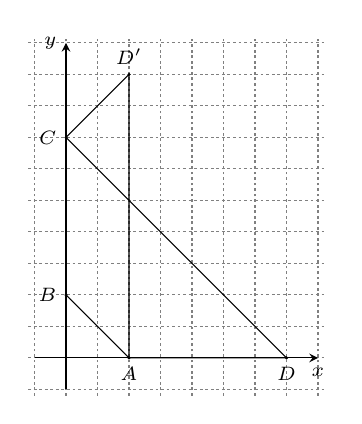
\begin{tikzpicture}[>=stealth,x=1cm,y=1cm,scale=0.4]
				\def\a{-2}
				\def\b{3}
				\draw[color=gray,dash pattern=on 1pt off 1pt,xstep=1.0cm,ystep=1.0cm] (-1.2,-1.2) grid (8.2,10.2);
				\draw[->] (-1,0) -- (8,0) node[below] {\scriptsize $x$};
				\draw[->] (0,-1) -- (0,10) node[left] {\scriptsize $y$};
				\coordinate[label=below:\scriptsize $A$] (A) at (2,0);
				\coordinate[label=left:\scriptsize $B$] (B) at (0,2);
				\coordinate[label=left:\scriptsize $C$] (C) at (0,7);
				\coordinate[label=below:\scriptsize $D$] (D) at (7,0);
				\coordinate[label=above:\scriptsize $D'$] (D') at (2,9);
				\draw (A)--(B)--(C)--(D)--(A) (A)--(B)--(C)--(D')--(A) ;
				\foreach \diem in {A,B,C,D,D'}	\fill (\diem)circle(1.5pt);
			\end{tikzpicture}	
		\end{center}
		Trường hợp 1: Hình thang có hai đáy $A B$, $C D$.\\
		Ta có $\heva{&\overrightarrow{AB},\overrightarrow{CD}\text{ cùng phương}\\&AD=BC}\Leftrightarrow\heva{&\dfrac{x}{-2}=\dfrac{y-7}{2} \\&\sqrt{(x-2)^2+y^2}=5} \Leftrightarrow\heva{&x=-y+7 \\&(-y+7-2)^2+y^2=25}$\\
		$\Leftrightarrow\heva{&x=-y+7 \\&2 y^2-10 y+25=25} \Leftrightarrow\heva{&x=7 \\&y=0} \vee\heva{&x=2 \\&y=5.}$\\
		Với $\heva{&x=7 \\&y=0}$ thì $CD=\sqrt{7^2+(0-7)^2}=7 \sqrt{2} \neq AB$ nên $D(7; 0)$ thỏa mãn.\\Với $\heva{&x=2 \\&y=5}$ thì $CD=\sqrt{2^2+(5-7)^2}=2 \sqrt{2}=AB$ (loại).\\Trường hợp 2: Hình thang có hai đáy $B C$, $A D$. Làm tương tự, ta có được điểm $D(2; 9)$.\\
		Giá trị nhỏ nhất của $a+b$ là $7$.
	}
\end{ex}
\begin{ex}%[0H9H1-6]
	Cho $\Delta AB C$ có $A(5; 6)$, $B(4;-1)$, $C(-4; 3)$. Tọa độ điểm $M(a;b)$ thuộc đoạn $BC$ sao cho $S_{\Delta MAB}=5 S_{\Delta MAC}$. Khi đó $a+b$ gần bằng
	\shortans{$-0{,}3$}
	\loigiai{
		\begin{center}
			\begin{tikzpicture}[scale=1, font=\footnotesize, line join=round, line cap=round, >=stealth]
				\def\a{4}
				\coordinate[label=left:\scriptsize $B$] (B) at (0,0);
				\coordinate[label=right:\scriptsize $C$] (C) at (\a,0);
				\coordinate[label=above:\scriptsize $A$] (A) at ($(B)+(65:.75*\a)$);
				\coordinate[label=below:\scriptsize $H$] (H) at ($(B)!(A)!(C)$);
				\coordinate[label=below:\scriptsize $M$] (M) at ($(C)!1/6!(B)$);
				\draw (M)--(A)--(B)--(C)--(A)--(H) ;
				\foreach \diem in {A,B,C,M,H}	\fill (\diem)circle(1.5pt);
				\newcommand{\gocv}[4][black]{\draw[#1] ($(#3)!5pt!(#2)$)--($(#3)!2!($($(#3)!5pt!(#2)$)!.5!($(#3)!5pt!(#4)$)$)$)--($(#3)!5pt!(#4)$);}
				\gocv{A}{H}{C}
			\end{tikzpicture}
		\end{center}
		Kẻ $AH \perp BC$. $S_{\Delta MAB}=5 S_{\Delta MAC}\Leftrightarrow \dfrac{1}{2}AH\cdot MB=5\cdot \dfrac{1}{2}AH\cdot MC\Leftrightarrow MB=5MC$. \\Mà $\overrightarrow{M B}$ và $\overrightarrow{M C}$ ngược hướng $\Rightarrow \overrightarrow{M B}=-5 \overrightarrow{M C}$ \\ $\Leftrightarrow \heva{&x_B-x_M=-5(x_C-x_M)\\&y_B-y_M=-5(y_C-y_M)}\Leftrightarrow\heva{& 4-x_M=-5(-4-x_M)\\&-1-y_M=-5(3-y_M)}\Rightarrow M\left(-\dfrac{8}{3};\dfrac{7}{3}\right)$.\\
		Suy ra $a+b=-\dfrac{1}{3}\approx-0{,}3$.	
	}
\end{ex}
\begin{ex}%[0H9H1-4]
	Cho $\vec{u}=(2 x-1; 3)$, $\vec{v}=(1; x+2)$. Có hai giá trị của $x$ để $\vec{u}$ cùng phương với $\vec{v}$. Tính tích hai giá trị đó.
	\shortans{$-2{,}5$}
	\loigiai{
		Với $x=-2$: Ta có $\vec{u}=(-5; 3); \vec{v}=(1; 0)$.\\
		Vì $\dfrac{1}{-5} \neq \dfrac{0}{3}$ nên hai véc-tơ $\vec{u}; \vec{v}$ không cùng phương.\\
		Với $x \neq-2$, ta có $\vec{u}; \vec{v}$ cùng phương khi và chỉ khi $$\dfrac{2 x-1}{1}=\dfrac{3}{x+2}\Leftrightarrow(2 x-1)(x+2)=3 \Leftrightarrow 2 x^2+3 x-5=0 \Leftrightarrow\hoac{&x=1 \\& x=-\dfrac{5}{2}.}$$
		Vậy tích của chúng là $1 \cdot\left(-\dfrac{5}{2}\right)=-2{,}5$.	
	}
\end{ex}
\begin{ex}%[0H9C1-3] 
	Cho ba điểm $A(-1; 4)$, $B(1; 1)$, $C(3;-1)$. Điểm $N(a;0)$ thuộc trục hoành sao cho $|N A-N C|$ bé nhất. Giá trị $a$ gần bằng
	\shortans{$4{,}33$}
	\loigiai{
		Ta thấy $y_A \cdot y_C=4 \cdot(-1)<0$ nên $A$, $C$ nằm khác phía so với trục $O x$.\\
		Lấy điểm $C$ đối xứng với $C$ qua $Ox$. Suy ra $C(3;1)$ và $C$, $A$ cùng phía so với $Ox$.\\
		Ta có $N\in Ox\Rightarrow NC=NC$. Vì vậy $\left| NA-NC\right|=\left| NA-NC\right|\le AC$.\\
		Suy ra $\left| NA-NC\right|_{\max}=AC$; giá trị lớn nhất này đạt được khi $A$, $C$, $N$ thẳng hàng ($N$ nằm ngoài $A$, $C$).\\
		Gọi $N(a;0)\in Ox\Rightarrow \overrightarrow{AN}=(a+1;-4)$, $\overrightarrow{AC}=(4;-3)$.\\
		Vì $\overrightarrow{AN}$, $\overrightarrow{AC}$ cùng phương nên $\dfrac{a+1}{4}=\dfrac{-4}{-3} \Leftrightarrow-3 a-3=-16 \Leftrightarrow a=\dfrac{13}{3}\approx4{,}33$.
	}
\end{ex}
\begin{ex}%[0H9C1-3] 
	Trong mặt phẳng tọa độ $Oxy$, cho hình bình hành $ABCD$ có $A(4;3)$, $C(8;1)$. Gọi $M$ là trung điểm của cạnh $BC$, $N$ là giao điểm của $BD$ và $AM$. Tính tổng hoành độ của các đỉnh còn lại của hình bình hành $ABCD$, biết $N\left(\dfrac{13}{3};2\right)$.
	\shortans{$11$}
	\loigiai{
		\begin{center}
			\begin{tikzpicture}[scale=1, font=\footnotesize, line join=round, line cap=round, >=stealth]
				\def\a{6}
				\coordinate[label=left:\scriptsize $B$] (B) at (0,0);
				\coordinate[label=right:\scriptsize $C$] (C) at (\a,0);
				\coordinate[label=above:\scriptsize $A$] (A) at ($(B)+(55:.45*\a)$);
				\coordinate[label=above:\scriptsize $D$] (D) at ($(C)-(B)+(A)$);
				\coordinate[label=above:\scriptsize $I$] (I) at ($(C)!.5!(A)$);
				\coordinate[label=below:\scriptsize $M$] (M) at ($(C)!.5!(B)$);
				\coordinate[label=above:\scriptsize $N$] (N) at ($(M)!1/3!(A)$);
				\draw (M)--(A)--(B)--(C)--(D)--(A)--(C) (D)--(B);
				\foreach \diem in {A,B,C,D,M,N,I}	\fill (\diem)circle(1.5pt);
			\end{tikzpicture}
		\end{center}
		Vì $I$ là tâm của hình bình hành $ABCD$.\\
		Nên $I$ là trung điểm của $AC$ suy ra $\heva{&x_I=\dfrac{3+8}{2}=\dfrac{11}{2}\\&y_I=\dfrac{4+1}{2}=\dfrac{5}{2}}\Rightarrow I\left(\dfrac{11}{2};\dfrac{5}{2}\right)$.\\
		Xét tam giác $ABC$ thì $BI$, $AM$ là hai đường trung tuyến nên $N$ là trọng tâm tam giác $ABC$.\\
		Do đó $\heva{&\dfrac{13}{3}=\dfrac{3+x_B+8}{3}\\&2=\dfrac{4+y_B+1}{3}}\Leftrightarrow\heva{&x_B=2\\&y_B=1}\Rightarrow B(2;1)$.\\
		Gọi $D(x_D;y_D)$. Do $I$ trung điểm của $BD\Rightarrow\heva{&2+x_D=11\\&1+y_D=5}\Leftrightarrow\heva{&x_D=9\\&y_D=4}$
		nên $D(9;4)$.\\
		Vậy tổng hoành độ của các đỉnh còn lại của hình bình hành $ABCD$ bằng $11$.
	}
\end{ex}

\Closesolutionfile{ans}
\indapan{6}{ans/ans-0-B1-KQ}
\newpage 
\subsection{Đề 2}
\Opensolutionfile{ans}[ans/ans-0-B1]
\caulc
%cau 1
\begin{ex}%[0H9N1-3]
Trong mặt phẳng $Oxy$, cho $A(5 ; 2)$, $B(10 ; 8)$. Toạ độ của $\vv{AB}$ là	
\choice
{$(2 ; 4)$}
{\True $(15 ; 10)$}
{$(50 ; 16)$}
{$(5 ; 6)$}
\loigiai{
Ta có $A(5 ; 2)$, $B(10 ; 8)$ nên $ \vv{AB} = (15 ; 10) $.
}
\end{ex}

%cau 2
\begin{ex}%[0H9N1-3]
Trong hệ tọa độ $Oxy$, cho $\vec{u}=\dfrac{1}{2} \vec{i}-5 \vec{j}$. Tọa độ vectơ $\vec{u}$ là
\choice
{$\vec{u}=\left(\dfrac{1}{2} ; 5\right)$}
{\True $\vec{u}=\left(\dfrac{1}{2} ;-5\right)$}
{$\vec{u}=(-1 ; 10)$}
{$\vec{u}=(1 ;-10)$}
\loigiai{
Ta thấy
$$
	\vec{u}=\dfrac{1}{2} \vec{i}-5 \vec{j}
	\Rightarrow
	\vec{u}=\left(\dfrac{1}{2} ;-5\right).
$$
}
\end{ex}

%cau 3
\begin{ex}%[0H9H1-4]
Trong mặt phẳng với hệ trục tọa độ $Oxy$, cho vecto $\vec{a}=(1 ;-2)$. Trong các vectơ dưới đây, vectơ nào cùng phương với $\vec{a}$.
\choice
{$\vec{b}=(1 ; 2)$}
{$\vec{c}=(-1 ;-2)$}
{\True $\vec{d}=(-2 ; 4)$}
{$\vec{e}=(2 ; 1)$}
\loigiai{
Ta có $\vec{d}=(-2 ; 4)=-2(1 ;-2)=-2 \vec{a}$. Do đó, $\vec{d}$ cùng phương với $\vec{a}$.
}
\end{ex}

%cau 4
\begin{ex}%[0H9H1-3]
Trong mặt phẳng toạ độ $Oxy$, cho hai điểm $A(1 ;-3)$, $B(3 ; 1)$. Toạ độ trung điểm $I$ của đoạn thẳng $AB$ là
\choice
{$I(-1 ;-2)$}
{\True $I(2 ;-1)$}
{$I(1 ;-2)$}
{$I(2 ; 1)$}
\loigiai{
Toạ độ trung điểm $I$ của đoạn thẳng $AB$ là
$$
	\heva{&x_I = \dfrac{x_A+x_B}{2}=2 \\ &y_I = \dfrac{y_A+y_B}{2}=-1}
$$
Vậy $I(2 ;-1)$.
}
\end{ex}

%cau 5
\begin{ex}%[0H9H1-3]
Trong mặt phẳng $Oxy$ cho $A(-2 ; 0)$, $B(5 ;-4)$. Tọa độ điểm $E$ đối xứng với $A$ qua $B$ là
\choice
{$E(-9 ; 4)$}
{$E(12 ; 8)$}
{\True $E(12 ;-8)$}
{$E(-8 ; 12)$}
\loigiai{
Điểm $E$ đối xứng với $A$ qua $B$ nên $B$ là trung điểm của đoạn $A E$.
Do đó
$$
	\heva{&x_E=2 x_B-x_A=2 \cdot 5-(-2)=12; \quad
	 \\ &y_E=2 y_B-y_A=2 \cdot (-4)-0=-8.}
$$
Vậy $ E(12 ;-8) $.
}
\end{ex}

%cau 6
\begin{ex}%[0H9H1-3]
Trong mặt phẳng $Oxy$, cho hình bình hành $ABCD$ biết $A(2 ; 1)$, $B(2 ;-1)$, $C(-2 ;-3)$. Tọa độ giao điểm hai đường chéo của hình bình hành $ABCD$ là
\choice
{$(2 ; 0)$}
{$(2 ; 2)$}
{$(0 ;-2)$}
{\True $(0 ;-1)$}
\loigiai{
Giao điểm hai đường chéo $ I $ là trung điểm của $A C$.
$$
	\heva{&x_I = \dfrac{x_A+x_B}{2}=0 \\ &y_I = \dfrac{y_A+y_B}{2}=-1.}
$$
Vậy tọa độ giao điểm hai đường chéo là $I(0 ;-1)$.
}
\end{ex}

%cau 7
\begin{ex}%[0H9H1-3]
Trong hệ trục tọa độ $Oxy$, cho $A(-4 ; 1)$, $B(2 ; 4)$, $C(2 ;-2)$. Tọa độ trọng tâm $G$ của tam giác $ABC$ là
\choice
{$G\left(0 ; \dfrac{3}{2}\right)$}
{\True $G(0 ; 1)$}
{$G(0 ; 3)$}
{$G\left(\dfrac{3}{2} ; 0\right)$}
\loigiai{
$G$ là trọng tâm của tam giác $ABC$ nên ta có
$$	
	\heva{&x_G=\dfrac{-4+2+2}{3}=0 \\ &y_G=\dfrac{1+4-2}{3}=1.}
$$
Vậy $G(0 ; 1)$.
}
\end{ex}

%cau 8
\begin{ex}%[0H9N1-3]]
Trong mặt phẳng với hệ trục tọa độ $(O ; \vec{i} ; \vec{j})$ cho điểm $M$ thỏa mãn $\vv{O M}=-2 \vec{i}+3 \vec{j}$. Tọa độ của điểm $M$ là
\choice
{\True $(-2 ; 3)$}
{$(2 ;-3)$}
{$(3 ;-2)$}
{$(-3 ; 2)$}
\loigiai{
$\vv{O M}=-2 \vec{i}+3 \vec{j}$ nên tọa độ điểm $M$ là $(-2 ; 3)$.
}
\end{ex}

%cau 9
\begin{ex}%[0H9H1-3]
Trong hệ tọa độ $Oxy$, cho tam giác $ABC$ có $A(6 ; 1)$, $B(-3 ; 5)$ và trọng tâm $G(-1 ; 1)$. Tìm tọa độ đỉnh $C$?
\choice
{$C(6 ;-3)$}
{$C(-6 ; 3)$}
{\True $C(-6 ;-3)$}
{$C(-3 ; 6)$}
\loigiai{
Gọi $C(x ; y)$. Vì $G$ là trọng tâm tam giác $ABC$ nên 
$$
	\heva{&\dfrac{6+(-3)+x}{3}=-1 \\ &\dfrac{1+5+y}{3}=1}
	\Leftrightarrow
	\heva{&x=-6 \\ &y=-3.}
$$
}
\end{ex}

%cau 10
\begin{ex}%[0H9V1-3]
Trong hệ tọa độ $Oxy$, cho tam giác $ABC$ có $C(-2 ;-4)$, trọng tâm $G(0 ; 4)$ và trung điểm cạnh $B C$ là $M(2 ; 0)$. Tổng hoành độ của điểm $A$ và $B$ là
\choice
{$ -2 $}
{\True $ 2 $}
{$ 4 $}
{$ 8 $}
\loigiai{
Vì $M$ là trung điểm $B C$ nên 
$$
	\heva{&x_B=2 x_M-x_C=2.2-(-2)=6 \\ &y_B=2 y_M-y_C=2.0-(-4)=4}
	\Rightarrow B(6 ; 4).
$$
Vì $G$ là trọng tâm tam giác $ABC$ nên 
$$
	\heva{&x_A=3 x_G-x_B-x_C=-4 \\ &y_A=3 y_G-y_B-y_C=12}
	\Rightarrow A(-4 ; 12).
$$
Suy ra $x_A+x_B=2$.
}
\end{ex}

%cau 11
\begin{ex}%[0H9V1-3]
Trong hệ tọa độ $Oxy$, cho $A(1 ; 3)$, $B(4 ; 0)$, $C(2 ;-5)$. Tìm tọa độ điểm $M$ thỏa mãn hệ thức $\vv{M A}+\vv{M B}-3 \vv{M C}=\vv{0}$?
\choice
{$M(1 ; 18)$}
{$M(-1 ; 18)$}
{\True $M(1 ;-18)$}
{$M(-18 ; 1)$}
\loigiai{
Gọi tọa độ $M(x ; y)$.
\\
Suy ra $\vv{M A}=(1-x ; 3-y)$, $\vv{M B}=(4-x ;-y)$, $\vv{M C}=(2-x ;-5-y)$.
\\
Ta có 
$$
	\vv{M A}+\vv{M B}-3 \vv{M C}=\vv{0} 
	\Leftrightarrow
	\heva{&(1-x)+(4-x)-3(2-x)=0 \\ &3-y-y-3(-5-y)=0}
	\Leftrightarrow
	\heva{&x=1 \\ &y=-18.}
$$
}
\end{ex}

%cau 12
\begin{ex}%[0H9V1-3]
Trong hệ tọa độ $Oxy$, cho tam giác $ABC$ có $B(9 ; 7)$, $C(11 ;-1)$. Gọi $M, N$ lần lượt là trung điểm của $AB$, $A C$. Tìm tọa độ vectơ $\vv{M N}$?
\choice
{$\vv{M N}=(2 ;-8)$}
{\True $\vv{M N}=(1 ;-4)$}
{$\vv{M N}=(10 ; 6)$}
{$\vv{M N}=(5 ; 3)$}
\loigiai{
Dễ thấy $ MN $ là đường trung bình của tam giác $ ABC $ mà
$$
	\vv{B C}=(2 ;-8) \quad \text{nên} \quad
	\vv{M N}=\dfrac{1}{2} \vv{B C}=(1 ;-4)
$$
}
\end{ex}


\Closesolutionfile{ans}
\indapan{6}{ans/ans-0-B1}


\cauds
\Opensolutionfile{ans}[ans/ans-0-B1-DS]
%cau 1
\begin{ex}%[0H9V1-3]
Trong mặt phẳng toạ độ  $ Oxy $, cho  $ A(-2 ; 5) $, $ B(-4 ;-2) $, $ C(1 ; 5) $. Các mệnh đề sau đúng hay sai?
\choiceTF
{\True Ba điểm $A, B, C$ không thẳng hàng}
{\True $G\left(-\dfrac{5}{3} ; \dfrac{8}{3}\right)$ là tọa độ trọng tâm của tam giác $ABC$}
{Tứ giác $ABCD$ là hình bình hành khi đó tọa độ điểm $D$ là $D(3 ; 10)$}
{$ \widehat{A C B}=45^{\circ} $}
\loigiai{
\begin{itemchoice}
	\itemch
	Ta có $\vv{AB}=(-2 ;-7)$, $\vv{A C}=(3 ; 0)$.
	\\
	Do $\dfrac{3}{-2} \neq \dfrac{0}{-7}$ nên $\vv{AB}$, $\vv{A C}$ không cùng phương. Vì vậy ba điểm $A, B, C$ không thẳng hàng.
	
	\itemch 
	Do $ G $ là trọng tâm của tam giác  $ ABC $ nên tọa độ $ G $ là
	$$
		\heva{&x_G = \dfrac{x_A+x_B+x_C}{3} = -\dfrac{5}{3} \\ &y_G = \dfrac{y_A+y_B+y_C}{3} = \dfrac{8}{3}}
	$$
	Vậy $ G\left(-\dfrac{5}{3} ; \dfrac{8}{3}\right) $.
	
	\itemch 
	Giả sử $D(x ; y)$. Ta có $\vv{AB}=(-2 ;-7)$, $\vv{DC}=(1-x ; 5-y)$.
	\\
	Tứ giác $ABCD$ là hình bình hành nếu 
	$$
		\vv{AB}=\vv{DC}
		\Leftrightarrow
		\heva{&-2=1-x \\ &-7=5-y} 
		\Leftrightarrow
		\heva{&x=3 \\ &y=12}
	$$ 
	Vậy $D(3 ; 12)$.
	
	\itemch Ta có
	\begin{align*}
		&AB=\sqrt{(-2)^2+(-7)^2}=\sqrt{53}, \\
		&A C=\sqrt{[1-(-2)]^2+(5-5)^2}=3, \\
		&B C=\sqrt{[1-(-4)]^2+[5-(-2)]^2}=\sqrt{74}.
	\end{align*}
	Ta có
	$$
		\vv{CA} \cdot \vv{CB}=(-3) \cdot (-5) + 0 \cdot (-7)=15.
	$$
	Suy ra
	$$
		\cos \widehat{ACB}=\cos (\vv{CA} , \vv{CB})
		=\dfrac{\vv{CA} \cdot \vv{CB}}{|\vv{CA}| \cdot|\vv{CB}|}
		=\dfrac{15}{3 \cdot \sqrt{74}}
		=\dfrac{5}{\sqrt{74}}.
	$$
	nên $\widehat{ACB} \approx 54^{\circ}$.
\end{itemchoice}
}
\end{ex}

%cau 2
\begin{ex}%[0H9V1-3]
Cho $ \vec{a}=3 \vec{i}+\vec{j} $, $ \vec{b}=-2 \vec{j} $. Các mệnh đề sau đúng hay sai?
\choiceTF
{$ \vec{a}=(-3 ; 1) $}
{\True $ \vec{b}=(0 ;-2) $}
{$ \vec{a}+\vec{b}=(3 ; 1) $}
{$ \vec{a}-\vec{b}=(3 ;-3) $}
\loigiai{
\begin{itemchoice}
	\itemch Ta có $ \vec{a}=(3 ; 1) $.
	
	\itemch Ta có $ \vec{b}=(0 ;-2) $.
	
	\itemch Ta có $ \vec{a}+\vec{b}=(3 ; 1)+(0 ;-2)=(3 ;-1) $.
	
	\itemch Ta có $ \vec{a}-\vec{b}=(3 ; 1)-(0 ;-2)=(3 ; 3) $.
\end{itemchoice}
}
\end{ex}

%cau 3
\begin{ex}%[0H9V1-3]
Cho $ \vec{a}=\dfrac{1}{2} \vec{i}+2 \vec{j} $, $ \vec{b}=\vec{i}-\dfrac{1}{2} \vec{j} $. Các mệnh đề sau đúng hay sai?
\choiceTF
{$ \vec{a}=\left(\dfrac{1}{2} ;-2\right) $}
{\True $ \vec{b}=\left(1 ;-\dfrac{1}{2}\right) $}
{\True $ 2 \vec{a}+3 \vec{b}=\left(4 ; \dfrac{5}{2}\right) $}
{\True $ \vec{a}-2 \vec{b}=\left(-\dfrac{3}{2} ; 3\right) $}
\loigiai{
\begin{itemchoice}
	\itemch Ta có $ \vec{a}=\left(\dfrac{1}{2} ; 2\right) $.
	
	\itemch Ta có $ \vec{b}=\left(1 ;-\dfrac{1}{2}\right) $.
	
	\itemch Ta có
	$$
		\heva{&2 \vec{a}=(1 ; 4) \\
			&3 \vec{b}=\left(3 ;-\dfrac{3}{2}\right)}
		\Rightarrow 
		2 \vec{a}+3 \vec{b}=\left(4 ; \dfrac{5}{2}\right)
	$$
	
	\itemch Ta có
	$$
		\heva{&\vec{a}=\left(\dfrac{1}{2} ; 2\right) \\
			&-2 \vec{b}=(-2 ; 1)}
		 \Rightarrow
		 \vec{a}-2 \vec{b}=\left(-\dfrac{3}{2} ; 3\right).
	$$
\end{itemchoice}
}
\end{ex}

%cau 4
\begin{ex}%[0H9V1-3]
Trong mặt phẳng tọa độ $Oxy$, cho tam giác $ABC$ có các đỉnh thỏa mãn $\vv{O A}=2 \vec{i}-\vec{j}$, $\vv{O B}=\vec{i}+\vec{j}$, $\vv{O C}=4 \vec{i}+\vec{j}$. Các mệnh đề sau đúng hay sai?
\choiceTF
{\True $A(2 ;-1)$, $B(1 ; 1)$, $C(4 ; 1)$}
{\True $E$ là trung điểm $AB$ nên $E\left(\dfrac{3}{2} ; 0\right)$}
{$G$ là trọng tâm $\triangle ABC$ nên $G\left(\dfrac{2}{3} ; \dfrac{1}{3}\right)$}
{Điểm $D$ sao cho $ABCD$ là hình bình hành nên $D(2 ;-1)$}
\loigiai{
\begin{itemchoice}
	\itemch Ta có
	\begin{eqnarray*}
		&\vv{O A}=2 \vec{i}-\vec{j} \Rightarrow A(2 ;-1), \\
		&\vv{O B}=\vec{i}+\vec{j} \Rightarrow B(1 ; 1), \\
		&\vv{O C}=4 \vec{i}+\vec{j} \Rightarrow C(4 ; 1)
	\end{eqnarray*}
	
	\itemch $ E $ là trung điểm  $ AB $ nên 
	$$
		\heva{&x_E=\dfrac{x_A+x_B}{2}=\dfrac{2+1}{2}=\dfrac{3}{2}, \\
		&y_E=\dfrac{y_A+y_B}{2}=\dfrac{-1+1}{2}=0}
	$$ 
	hay $ E \left(\dfrac{3}{2} ; 0\right) $.
	
	\itemch $G$ là trọng tâm $\triangle ABC$ nên
	$$
		\heva{&x_G=\dfrac{x_A+x_B+x_C}{3}=\dfrac{2+1+4}{3}=\dfrac{7}{3}\\
		&y_G=\dfrac{y_A+y_B+y_C}{3}=\dfrac{-1+1+1}{3}=\dfrac{1}{3}.}
	$$
	hay $G\left(\dfrac{7}{3} ; \dfrac{1}{3}\right)$.
	
	\itemch Do $ABCD$ là hình bình hành nên
	$$
		\vv{A D}=\vv{B C} 
		\Leftrightarrow
		\heva{&x _ { D } - x _ { A } = x _ { C } - x _ { B } \\ &y _ { D } - y _ { A } = y _ { C } - y _ { B }}
		\Leftrightarrow 
		\heva{&x _ { D } - 2 = 4 - 1 \\ &y _ { D } + 1 = 1 - 1}
		\Leftrightarrow 
		\heva{&x_D=5 \\ &y_D=-1.}
	$$
	Vậy $D(5 ;-1)$.
\end{itemchoice}
}
\end{ex}

\Closesolutionfile{ans}
\indapan{3}{ans/ans-0-B1-DS}


\Opensolutionfile{ans}[ans/ans-0-B1-KQ]
\caukq
%cau 1
\begin{ex}%[0H9V1-3]
Trong mặt phẳng tọa độ $Oxy$, cho hai điểm $M(5 ; 3), N(-3 ; 5)$. Điểm $P$ nằm trên trục hoành sao cho ba điểm $M, N, P$ thẳng hàng. Hoành độ điểm $ P $ là bao nhiêu?
\shortans{$17$}
\loigiai{
$P$ là điểm nằm trên trục hoành nên $P(x, 0)$.
\\
Ta có $\vv{M N}=(-8 ; 2) ; \vv{M P}=(x-5 ;-3)$.
\\
Ba điểm $M, N, P$ thẳng hàng khi
$$
	\vv{M P}=k \vv{M N} 
	\Leftrightarrow
	\heva{&x-5=k \cdot(-8) \\ &-3=k \cdot 2}
	\Leftrightarrow
	\heva{&x=17 \\ &k=-\dfrac{3}{2}.}
$$ 
Vậy $x_P=17$.
}
\end{ex}

%cau 2
\begin{ex}%[0H9H1-3]
Trong mặt phẳng toạ độ $Oxy$, cho $\vec{a}=(m ; 2)$, $\vec{b}=(-3 ; n)$ và $\vec{c}=(-2 m ; 7)$. Tìm $m+n$ biết $\vec{c}=\vec{a}+\vec{b}$.
\shortans{$6$}
\loigiai{
Ta có
$$
	\vec{c}=\vec{a}+\vec{b} 
	\Leftrightarrow
	\heva{&-2 m=m-3 \\ &7=2+n}
	\Leftrightarrow
	\heva{&m=1 \\ &n=5.}
$$
Vậy $m+n=6$.
}
\end{ex}

%cau 3
\begin{ex}%[0H9H1-3]
Trong mặt phẳng toạ độ $Oxy$, cho $A(2 ; 2)$, $B(1 ;-3)$, $C(-3 ; 0)$. Điểm $E$ thoả mãn $\vv{A E}=-2 \vv{AB}+3 \vv{A C}$. Khi đó giá trị của $ x_E \cdot y_E $ là bao nhiêu?
\shortans{$-66$}
\loigiai{
Giả sử $E(x ; y)$.
Ta có
$$
	\vv{A E}=(x-2 ; y-2), \quad
	\vv{AB}=(-1 ;-5), \quad
	\vv{A C}=(-5 ;-2).
$$
Suy ra
$$
	-2 \vv{AB}+3 \vv{A C}=(-13 ; 4).
$$
Do đó
$$
	\vv{A E}=-2 \vv{AB}+3 \vv{A C} 
	\Leftrightarrow
	\heva{&x-2=-13 \\ &y-2=4}
	\Leftrightarrow
	\heva{&x=-11 \\ &y=6.}
$$
Vậy $x_E \cdot y_E = -66$.
}
\end{ex}

%cau 4
\begin{ex}%[0H9V1-3]
Trong mặt phẳng toạ độ $Oxy$, cho hai điểm $A(1 ; 5)$, $B(9 ; 3)$. Điểm $M$ thuộc trục hoành sao cho $\widehat{A M B}=90^{\circ}$. Có bao nhiêu điểm $ M $ thỏa mãn yêu cầu bài toán?
\shortans{$2$}
\loigiai{
Điểm $M$ thuộc trục hoành nên giả sử $M(m ; 0)$.
\\
Ta có
$$
	\vv{M A}=(1-m ; 5), \quad
	\vv{M B}=(9-m ; 3).
$$
Theo đề bài
$$
	\widehat{A M B}=90^{\circ} 
	\Leftrightarrow 
	\vv{M A} \cdot \vv{M B}=0 
	\Leftrightarrow(1-m)(9-m)+5 \cdot 3=0
	\Leftrightarrow m^2-10 m+24=0 
	\Leftrightarrow
	\hoac{&m=6 \\ &m=4.}
$$
Vậy có $ 2 $ trường hợp điểm $M$ thoả mãn bài toán là: $M(4 ; 0)$ và $M(6 ; 0)$.
}
\end{ex}

%cau 5
\begin{ex}%[0H9V1-3]
Trong mặt phẳng toạ độ $Oxy$, cho hai điểm $A(4 ;-2)$ và $B(10 ; 4)$. Điểm $M$ trên trục tung sao cho $|\vv{M A}+\vv{M B}|$ đạt giá trị nhỏ nhất. Tung độ của điểm $ M $ có giá trị bao nhiêu?
\shortans{$1$}
\loigiai{
Điểm $M$ thuộc trục tung nên giả sử $M(0 ; m)$.
Ta có
$$
	\vv{M A}=(4 ;-2-m), \quad
	\vv{M B}=(10 ; 4-m).
$$
Suy ra 
$$
	\vv{M A}+\vv{M B}=(14 ; 2-2 m)
$$
Do đó
$$
	|\vv{M A}+\vv{M B}|
	=\sqrt{14^2+(2-2 m)^2} \geq 14.
$$
Dấu bằng xảy ra khi $m=1$.
\\
Vậy $|\vv{M A}+\vv{M B}|$ đạt giá trị nhỏ nhất bằng $ 14 $ khi $M$ có toạ độ là $(0 ; 1)$.
}
\end{ex}

%cau 6
\begin{ex}%[0H9V1-3]
Cho các vectơ $\vec{a}=(1 ;-2)$, $\vec{b}=(-2 ;-6)$, $\vec{c}=(m+n ;-m-4 n)$.
Tồn tại hai số thực $m, n$ sao cho $\vec{c}$ cùng phương $\vec{a}$ và $|\vec{c}|=3 \sqrt{5}$. Khi đó giá trị của biểu thức $ |m+n| $ là bao nhiêu?
\shortans{$ 3 $}
\loigiai{
$ \vec{c} $ cùng phương $ \vec{a} $ và $ |\vec{c}|=3 \sqrt{5} $ nên
\begin{align*}
	\heva{&\dfrac{m+n}{1}=\dfrac{-m-4 n}{-2} \\ &\sqrt{(m+n)^2+(-m-4 n)^2}=3 \sqrt{5}}
	&\Leftrightarrow
	\heva{&- 2 m - 2 n = - m - 4 n \\ &( m + n ) ^ { 2 } + ( m + 4 n ) ^ { 2 } = 4 5} \\
	&\Leftrightarrow
	\heva{&m = 2 n \\ &( 3 n ) ^ { 2 } + ( 6 n ) ^ { 2 } = 4 5} \\
	&\Leftrightarrow
	\heva{&m=2 n \\ &4 5 n ^ { 2 } = 4 5} \\
	&\Leftrightarrow
	\heva{&m=2 \\ &n=1} \vee \heva{&m=-2 \\ &n=-1.}
\end{align*}
Trong cả hai trường hợp, ta đều thấy $ |m+n| = 3 $.
}
\end{ex}
\Closesolutionfile{ans}
\indapan{6}{ans/ans-0-B1-KQ}